\documentclass[11pt,a4paper]{article}

% --- Paquetes de Estilo y Formato ---
\usepackage[utf8]{inputenc}
\usepackage[spanish,es-tabla]{babel}
\usepackage[T1]{fontenc}
\usepackage{geometry}
\geometry{top=3cm, bottom=3cm, left=3cm, right=2.5cm}
\usepackage{tabularx}
\usepackage{titlesec}
\usepackage{fancyhdr}
\usepackage{lastpage}
\usepackage{hyperref}
\usepackage{enumitem}
\usepackage{graphicx}
\usepackage{tikz}
\usepackage{float}
\usepackage{array}
\usepackage{colortbl}
\usepackage[table, xcdraw]{xcolor}

% --- Definición de Colores Corporativos ArthroDesign ---
\definecolor{ArthroNavy}{HTML}{0F172A}
\definecolor{ArthroTeal}{HTML}{0D9488}
\definecolor{ArthroGray}{HTML}{64748B}
\definecolor{tabblue}{RGB}{173, 204, 230}

% --- Configuración de Párrafo ---
\setlength{\parskip}{0.5em}
\setlength{\parindent}{1.5em}

% --- Estilo de Títulos con Identidad Corporativa ---
\titleformat{\section}
  {\color{ArthroNavy}\Large\bfseries}
  {\thesection.}
  {0.5em}
  {}
  [{\color{ArthroTeal}\titlerule[1.5pt]}]

\titleformat{\subsection}
  {\color{ArthroNavy}\large\bfseries}
  {\thesubsection.}
  {0.5em}
  {}
  [{\color{ArthroTeal}\titlerule[1pt]}]

\titleformat{\subsubsection}
  {\color{ArthroNavy}\large\bfseries}
  {\thesubsubsection.}
  {0.5em}
  {}

% --- Viñetas en color Turquesa ---
\renewcommand{\labelitemi}{\color{ArthroTeal}\textbullet}
\renewcommand{\labelitemii}{\color{ArthroTeal}\circ}

% --- Configuración de Enlaces ---
\hypersetup{colorlinks=true, linkcolor=ArthroNavy, urlcolor=ArthroTeal}

% --- CONFIGURACIÓN DE ENCABEZADO Y PIE CORPORATIVO (Anexo I) ---
\pagestyle{fancy}
\fancyhf{}

% Línea superior de color turquesa (Grosor 2pt)
\renewcommand{\headrule}{\hbox to\headwidth{\color{ArthroTeal}\leaders\hrule height 2pt\hfill}}

% Información de Encabezado
\fancyhead[L]{\small \textbf{\color{ArthroNavy}Adaptador ergonómico - PR-PIB-GIS26-09}}
\fancyhead[R]{\small \textbf{\color{ArthroNavy}Anexo IV: Entrevistas y encuestas}}

% Información de Pie de Página
\fancyfoot[L]{\small \color{ArthroGray}ArthroDesign Solutions S.L.}
\fancyfoot[C]{\small \color{ArthroGray}\today}
\fancyfoot[R]{\small \textbf{\color{ArthroNavy}Pág. \thepage \ de \pageref{LastPage}}}

\setlength{\headheight}{15pt}
\renewcommand{\footrulewidth}{0.4pt}

\begin{document}

% ======================================================
% PÁGINA 1: PORTADA TÉCNICA (BLOQUE SÓLIDO)
% ======================================================
\begin{titlepage}
    
    % --- LOGO CORPORATIVO (Alineado a la derecha) ---
    \begin{flushright}
        \vspace*{-2cm}
        
\includegraphics[width=7.5cm]{logo_definitivo.png}
    \end{flushright}

    \vspace{-0.5cm}

    \begin{flushleft}
        % --- ETIQUETA DEL VOLUMEN ---
        {\color{ArthroGray}\Large \textbf{DOCUMENTO Nº 3: ANEXOS}} \\[0.5cm]
        
        % --- BLOQUE SÓLIDO DE IDENTIFICACIÓN DEL ANEXO ---
        \noindent\colorbox{ArthroNavy}{%
            \parbox{\dimexpr\textwidth-2\fboxsep\relax}{%
                \vspace{0.5cm}
                \centering
                \hspace{0.2cm}{\color{white}\fontsize{42pt}{48pt}\selectfont\textbf{ANEXO IV}}
                \vspace{0.5cm}
            }%
        } \\[0.8cm]
        
        % --- TÍTULO DEL ANEXO ---
        \centering
        {\color{ArthroTeal}\Huge\bfseries ENTREVISTAS Y ENCUESTAS} \\[0.4cm]
        {\color{ArthroGray}\rule{\textwidth}{1.5pt}} \\
        
        \vspace{0.6cm}

        % --- INFORMACIÓN DEL PROYECTO MAESTRO ---
        \centering
        {\color{ArthroNavy}\small\textbf{TÍTULO DEL PROYECTO:}} \\[0.3cm]
        {\huge\bfseries Diseño de un adaptador ergonómico universal para la optimización de la pulsación manual en inhaladores de dosis medida (MDI)} \\
        
        \vspace{1cm}

        % --- BLOQUE DE IDENTIFICACIÓN TÉCNICA ---
                \centering
                {\color{ArthroGray}\small\textbf{CÓDIGO DE IDENTIFICACIÓN:}} \\ {\large\texttt{PR-PIB-GIS26-09}} \\
                \vspace{0.5cm}
                {\color{ArthroGray}\small\textbf{PROMOTOR Y EMPRESA DESARROLLADORA:}} \\ {\large ArthroDesign Solutions S.L.} \\{Calle Severo Ochoa, Nº 12, 29590 Málaga, España}\\
        {NIF: B12345678} \\
        \href{mailto:contacto@arthrodesign.com}{contacto@arthrodesign.com} \\
  

        \vspace{1cm}

        % --- BLOQUE DE PROYECTISTAS AUTORES ---
        {\color{ArthroNavy}\small\textbf{PROYECTISTAS (Equipo de ArthroDesign Solutions S.L.):}} \\[0.3cm]
        \small
        \renewcommand{\arraystretch}{1.4}
        \begin{tabular}{@{}l l}
            \textbf{D. Sergio Carmona Muñoz} & Colegiado Nº 06424 (DNI: 26291930D) \\
            \textbf{D. Juan Gabriel Navarro Valdivielso} & Colegiado Nº 06425 (DNI: 77666662D) \\
            \textbf{D. Antonio Sánchez Doña} & Colegiado Nº 06423 (DNI: 79380534J) \\
            \textbf{D. Iván de la Torre Segato} & Colegiado Nº 06421 (DNI: 79383630G) \\
        \end{tabular}

        \vfill

        % --- PIE DE PORTADA ---
        {\color{ArthroTeal}\rule{\linewidth}{1pt}} \\[0.3cm]
        \small\color{ArthroGray}  ArthroDesign Solutions S.L. \quad | \quad \today
    \end{flushleft}
\end{titlepage}

% AÑADE ESTA LÍNEA AQUÍ PARA QUE LA SIGUIENTE PÁGINA SEA LA 2:
\setcounter{page}{2}

% ======================================================
% HOJA EN BLANCO CON MARCA DE AGUA
% ======================================================
\newpage
\pagestyle{fancy}

\begin{tikzpicture}[remember picture, overlay]
    \node[opacity=0.1] at (current page.center) {
\includegraphics[width=12cm]{logo_definitivo.png}};
\end{tikzpicture}

% Empujamos el texto hacia la parte inferior del folio
\vspace*{8.5cm} 
\begin{center}
    \textit{Esta hoja ha sido dejada deliberadamente en blanco.}
\end{center}
\vfill
\newpage

% ======================================================
% PÁGINA: ÍNDICE AUTOMÁTICO (CON ENCABEZADO)
% ======================================================
\markboth{Índice}{Índice}
\tableofcontents
\thispagestyle{fancy} % Fuerza el estilo fancy en esta página
\newpage

% ======================================================
% PÁGINA: ÍNDICE DE TABLAS
% ======================================================
\markboth{Índice de tablas}{Índice de tablas}
\listoftables
\thispagestyle{fancy}
\newpage





\section{PERFIL DE CLIENTE SELECCIONADO}





\vspace{0.3cm}

\begin{table}[H]
    \centering
    \small
    \renewcommand{\arraystretch}{1.6} % Mayor holgura vertical para que respire el texto
    \renewcommand{\tabularxcolumn}[1]{m{#1}} % Centrado vertical de las celdas X
    % Alineación izquierda (\raggedright) en la 1ª columna para evitar bordes irregulares
    \begin{tabularx}{\linewidth}{>{\color{ArthroNavy}\bfseries\raggedright\arraybackslash}m{3.5cm} X}
        \hline
        \rowcolor{ArthroNavy}
        % Mantenemos los títulos centrados para la estética de la cabecera
        \multicolumn{1}{>{\centering\arraybackslash}m{3.5cm}}{\color{white}\textbf{Perfil de Usuario}} & 
        \multicolumn{1}{>{\centering\arraybackslash}X}{\color{white}\textbf{Descripción y Limitación Física}} \\ \hline
        
        \rowcolor{ArthroTeal!5}
        Perfil 1: \newline Patologías articulares & Pacientes diagnosticados con \textbf{Artritis Reumatoide o artrosis severa} en las manos. Para este grupo, la acción de presionar el inhalador estándar resulta mecánicamente dolorosa o totalmente imposible. \\
        
        Perfil 2: \newline Población geriátrica & Pacientes de la tercera edad con \textbf{sarcopenia}. Debido a la pérdida natural de masa y fuerza muscular, no pueden alcanzar el pico de fuerza necesario para liberar la dosis de su medicación respiratoria. \\ \hline
        
        \rowcolor{ArthroTeal!15} % Tono ligeramente más intenso para destacar la conclusión
        \multicolumn{2}{c}{
            \parbox[c]{\dimexpr\linewidth-2\tabcolsep\relax}{
                \vspace{0.3cm}
                \centering \textbf{\color{ArthroNavy}Valor Aportado General} \\ \vspace{0.15cm}
                Para ambos perfiles, el adaptador garantiza la administración correcta de la dosis diaria y representa una \textbf{recuperación de su autonomía personal}, eliminando la dependencia de terceros.
                \vspace{0.3cm}
            }
        } \\ \hline
    \end{tabularx}
    \caption{Definición de los perfiles de clientes críticos seleccionados para el desarrollo del producto.}
    \label{tab:perfil_cliente}
\end{table}
\section{ENTREVISTA A USUARIOS}

\subsection{Generación de preguntas: Propuestas individuales}

\vspace{0.4cm}

% --- TABLA 1: ANTONIO ---
\begin{table}[H]
    \centering
    \small
    \renewcommand{\arraystretch}{1.5}
    \begin{tabularx}{\linewidth}{|X|}
        \hline
        \rowcolor{ArthroNavy}
        \textcolor{white}{\textbf{Propuestas de D. Antonio Sánchez Doña}} \\ \hline
        \rowcolor{ArthroTeal!5}
        \vspace{0.1cm}
        \begin{enumerate}[leftmargin=0.8cm, itemsep=0.2cm]
            \item ¿En qué escala del 1 al 10 describiría el dolor que siente en sus dedos al intentar presionar el inhalador durante un brote de artritis?
            \item ¿Ha sentido alguna vez que su tratamiento es ineficaz simplemente porque no es capaz de accionar el spray correctamente?
            \item ¿Qué adaptaciones caseras o ``trucos'' ha intentado aplicar al inhalador para facilitar su uso?
            \item Si existiera un accesorio que facilite la presión, ¿preferiría que fuera lo más pequeño posible o priorizaría que el agarre fuera muy grande y blando?
            \item ¿Cuánto tiempo tarda normalmente en lograr accionar el dispositivo desde que lo saca de su estuche?
        \end{enumerate}
        \vspace{0.1cm} \\ \hline
    \end{tabularx}
    \caption{Propuestas de preguntas para la entrevista - D. Antonio Sánchez Doña.}
    \label{tab:preguntas_antonio}
\end{table}

\vspace{0.4cm}

% --- TABLA 2: SERGIO ---
\begin{table}[H]
    \centering
    \small
    \renewcommand{\arraystretch}{1.5}
    \begin{tabularx}{\linewidth}{|X|}
        \hline
        \rowcolor{ArthroNavy}
        \textcolor{white}{\textbf{Propuestas de D. Sergio Carmona Muñoz}} \\ \hline
        \vspace{0.1cm}
        \begin{enumerate}[leftmargin=0.8cm, itemsep=0.2cm]
            \item ¿Podría describirme cómo es su rutina cuando necesita usar el inhalador? ¿Qué pasos del proceso le resultan más difíciles o le generan más incomodidad?
            \item ¿Ha llegado a necesitar la ayuda de otra persona para poder usar el inhalador? ¿Cómo le hace sentir esa situación?
            \item ¿Ha comentado alguna vez a su médico neumólogo, reumatólogo o farmacéutico que tiene dificultades para usar el inhalador? ¿Cuál fue su respuesta o recomendación?
            \item ¿Desde que le diagnosticaron la artritis, ha notado que usar el inhalador se ha ido complicando progresivamente? ¿Cómo ha cambiado su relación con el dispositivo?
            \item ¿Qué información o garantías necesitaría antes de incorporar un accesorio nuevo a su rutina de inhalación? ¿Qué le generaría desconfianza?
        \end{enumerate}
        \vspace{0.1cm} \\ \hline
    \end{tabularx}
    \caption{Propuestas de preguntas para la entrevista - D. Sergio Carmona Muñoz.}
    \label{tab:preguntas_sergio}
\end{table}

\vspace{0.4cm}

% --- TABLA 3: IVÁN ---
\begin{table}[H]
    \centering
    \small
    \renewcommand{\arraystretch}{1.5}
    \begin{tabularx}{\linewidth}{|X|}
        \hline
        \rowcolor{ArthroNavy}
        \textcolor{white}{\textbf{Propuestas de D. Iván de la Torre Segato}} \\ \hline
        \rowcolor{ArthroTeal!5}
        \vspace{0.1cm}
        \begin{enumerate}[leftmargin=0.8cm, itemsep=0.2cm]
            \item ¿Qué movimiento concreto le resulta más difícil: sujetarlo, colocarlo correctamente, presionar el cartucho o coordinar la pulsación con la inhalación?
            \item Cuando usa el inhalador, ¿siente que la forma o el tamaño del dispositivo le permite agarrarlo con seguridad, o nota que se le resbala?
            \item ¿En qué situaciones le resulta más complicado utilizar el inhalador: en casa, fuera de casa, durante una crisis respiratoria, por la mañana/noche o durante un brote?
            \item Si pudiera modificar una sola característica física para facilitar su uso, ¿cuál elegiría?
            \item ¿Le preocuparía que un accesorio acoplado aumentara demasiado su tamaño o dificultara llevarlo en el bolsillo, bolso o estuche habitual?
        \end{enumerate}
        \vspace{0.1cm} \\ \hline
    \end{tabularx}
    \caption{Propuestas de preguntas para la entrevista - D. Iván de la Torre Segato.}
    \label{tab:preguntas_ivan}
\end{table}

\vspace{0.4cm}

% --- TABLA 4: JUAN GABRIEL ---
\begin{table}[H]
    \centering
    \small
    \renewcommand{\arraystretch}{1.5}
    \begin{tabularx}{\linewidth}{|X|}
        \hline
        \rowcolor{ArthroNavy}
        \textcolor{white}{\textbf{Propuestas de D. Juan Gabriel Navarro Valdivielso}} \\ \hline
        \vspace{0.1cm}
        \begin{enumerate}[leftmargin=0.8cm, itemsep=0.2cm]
            \item Sobre su rutina actual, ¿cómo es su experiencia utilizando el inhalador en momentos de brote de su enfermedad motora? 
            \item Cuando siente rigidez o dolor muscular, ¿cuáles son sus estrategias para administrarse la dosis? ¿Pide ayuda? ¿Utiliza una superficie para presionar?
            \item ¿Ha habido algún momento que debido a las molestias haya dudado de haberse administrado la dosis correcta? ¿Cómo le hizo sentir? 
            \item Si hubiese un dispositivo que permitiese que ejerciera fuerza con toda la mano, ¿cree que cambiaría su percepción de él? 
            \item Si existiese dicho dispositivo, ¿cuál cree que sería el accesorio o pieza de éste que más le preocuparía? 
        \end{enumerate}
        \vspace{0.1cm} \\ \hline
    \end{tabularx}
    \caption{Propuestas de preguntas para la entrevista - D. Juan Gabriel Navarro Valdivielso.}
    \label{tab:preguntas_juan}
\end{table}
\newpage

\subsection{Cuestionario consensuado del equipo}


\vspace{0.8cm}

% --- INICIO DEL FORMULARIO TIPO ENCUESTA ---

\begin{center}
    \Large\textbf{\color{ArthroNavy}FORMULARIO DE ENTREVISTA DE NECESIDADES DEL USUARIO} \\
    \vspace{0.2cm}
    \rule{\linewidth}{1.5pt}
\end{center}
\vspace{0.2cm}

% Datos del paciente
\noindent
\textbf{Nombre y apellidos:} \hrulefill \\[-0.5em] \\
\textbf{Edad:} \makebox[3cm]{\hrulefill} \hspace{1cm} 
\textbf{Género:} \makebox[1.5cm]{Hombre \hfill $\square$} \hspace{0.5cm} \makebox[1.5cm]{Mujer \hfill $\square$} \hspace{0.5cm} \makebox[2cm]{Otro \hfill $\square$} \\[-0.5em] \\
\textbf{Patología diagnosticada:} \hrulefill 
\vspace{0.8cm}

% Pregunta 1
\noindent
\begin{tabularx}{\linewidth}{|X|}
\hline
\rowcolor{ArthroTeal}
\textcolor{white}{\textbf{1. ¿Qué movimiento concreto o paso del proceso le resulta más difícil y doloroso al utilizar el inhalador durante su rutina diaria?}} \\ \hline
\rule{0pt}{1.4cm} \\ % <--- Cambia este valor (3.5cm) para ajustar el recuadro
\hline
\end{tabularx}

\vspace{0.5cm}

% Pregunta 2
\noindent
\begin{tabularx}{\linewidth}{|X|}
\hline
\rowcolor{ArthroTeal}
\textcolor{white}{\textbf{2. Cuando siente rigidez o dolor articular, ¿qué estrategias, trucos caseros o ayuda externa utiliza para lograr administrarse la dosis?}} \\ \hline
\rule{0pt}{1.4cm} \\ 
\hline
\end{tabularx}

\vspace{0.5cm}

% Pregunta 3
\noindent
\begin{tabularx}{\linewidth}{|X|}
\hline
\rowcolor{ArthroTeal}
\textcolor{white}{\textbf{3. ¿Cómo le hace sentir el hecho de no poder accionarlo correctamente o dudar de si ha recibido la dosis adecuada por falta de fuerza?}} \\ \hline
\rule{0pt}{1.4cm} \\ 
\hline
\end{tabularx}

\vspace{0.5cm}

% Pregunta 4
\noindent
\begin{tabularx}{\linewidth}{|X|}
\hline
\rowcolor{ArthroTeal}
\textcolor{white}{\textbf{4. Si existiera un accesorio acoplado para facilitar la presión, ¿preferiría priorizar un tamaño muy pequeño para llevarlo consigo o un agarre grande y cómodo aunque ocupe más espacio?}} \\ \hline
\rule{0pt}{1.4cm} \\ 
\hline
\end{tabularx}

\vspace{0.5cm}

% Pregunta 5
\noindent
\begin{tabularx}{\linewidth}{|X|}
\hline
\rowcolor{ArthroTeal}
\textcolor{white}{\textbf{5. ¿Qué información, garantía o característica física necesitaría para confiar en un accesorio nuevo y añadirlo a su rutina médica?}} \\ \hline
\rule{0pt}{1.4cm} \\ 
\hline
\end{tabularx}

% --- FIN DEL FORMULARIO ---

\vspace{1cm}
\newpage
\subsection{Resultados de la entrevista: Análisis cualitativo}


\vspace{0.4cm}

% --- Ficha Clínica del Paciente ---
\begin{table}[H]
    \centering
    \small
    \renewcommand{\arraystretch}{1.4}
    \begin{tabularx}{\linewidth}{|>{\columncolor{ArthroNavy}\color{white}\bfseries}m{3.5cm} | X|}
        \hline
        \multicolumn{2}{|c|}{\cellcolor{ArthroNavy}\textcolor{white}{\textbf{PERFIL CLÍNICO DEL USUARIO ENTREVISTADO}}} \\ \hline
        Nombre y Edad & Doña Carmen Ruiz, 68 años. \\ \hline
        Ubicación & Málaga. \\ \hline
        Patología Principal & \textbf{Artritis Reumatoide} (diagnosticada hace 12 años) con deformidad moderada en las articulaciones interfalángicas. \\ \hline
        Patología Secundaria & Asma bronquial leve (usuaria habitual de inhaladores MDI). \\ \hline
    \end{tabularx}
    \label{tab:perfil_entrevistada}
\end{table}

\vspace{0.4cm}

% --- Resultados de la Entrevista ---
\begin{table}[H]
    \centering
    \small
    \renewcommand{\arraystretch}{1.6}
    \renewcommand{\tabularxcolumn}[1]{m{#1}}
    \begin{tabularx}{\linewidth}{|>{\columncolor{ArthroTeal!5}\bfseries\raggedright\arraybackslash}m{4.5cm} | X|}
        \hline
        \rowcolor{ArthroNavy}
        \multicolumn{1}{|c|}{\textcolor{white}{\textbf{Foco de la Pregunta}}} & \multicolumn{1}{c|}{\textcolor{white}{\textbf{Experiencia de Uso (Transcripción literal)}}} \\ \hline
        
        1. Dificultad principal \newline \textit{(Fase crítica y dolorosa)} & 
        ``Lo peor sucede al intentar hacer la forma de pinza con el dedo índice y el pulgar. Colocar la boca me resulta sencillo. El problema llega en el momento exacto de apretar el cartucho hacia abajo. Mis dedos no tienen fuerza suficiente y el plástico tan estrecho del inhalador me clava los bordes en la piel.'' \\ \hline
        
        2. Estrategias de uso \newline \textit{(Alternativas adoptadas)} & 
        ``A veces apoyo la base del inhalador en la mesa del comedor. Pongo las dos manos planas encima del bote y dejo caer el peso de mi cuerpo hacia adelante para empujar. Otras veces tengo que esperar a que llegue mi marido para que él me pulse el aparato mientras yo aspiro.'' \\ \hline
        
        3. Impacto emocional \newline \textit{(Frustración e inseguridad)} & 
        ``Me genera muchísima ansiedad. Cuando tengo sensación de ahogo necesito que el medicamento entre rápido. Si aprieto flojo y sale poca medicina, me asusto y vuelvo a intentarlo con dolor. Siento una pérdida de independencia enorme al depender de otra persona para algo tan básico.'' \\ \hline
        
        4. Preferencias físicas \newline \textit{(Tamaño vs. Ergonomía)} & 
        ``Prefiero un aparato grande. Mis manos ya no pueden agarrar cosas finas. Si el adaptador tiene un mango grueso y puedo apoyarme bien, me da igual que ocupe todo el bolso. Prefiero la comodidad antes que la estética.'' \\ \hline
        
        5. Requisitos de diseño \newline \textit{(Garantías de seguridad)} & 
        ``Necesito ver que encaja a la perfección y de manera firme. Me daría mucho miedo apretar y que la pieza de plástico resbalara y saliera disparada. Si noto que el material es resistente y el médico me confirma que no altera la salida del gas, lo usaría a diario con total seguridad.'' \\ \hline
    \end{tabularx}
    \caption{Transcripción cualitativa y hallazgos clave de la entrevista guiada presencial.}
    \label{tab:resultados_entrevista}
\end{table}
\newpage
\section{ENCUESTA DE MERCADO}
\subsection{Generación de preguntas cuantitativas: Propuestas individuales}


\vspace{0.4cm}

% --- TABLA 1: ANTONIO ---
\begin{table}[H]
    \centering
    \small
    \renewcommand{\arraystretch}{1.5}
    \begin{tabularx}{\linewidth}{|X|}
        \hline
        \rowcolor{ArthroNavy}
        \textcolor{white}{\textbf{Preguntas propuestas por el proyectista D. Antonio Sánchez Doña}} \\ \hline
        \rowcolor{ArthroTeal!5}
        \vspace{0.1cm}
        \begin{enumerate}[leftmargin=0.8cm, itemsep=0.2cm]
            \item ¿Cuántas veces al día utiliza su inhalador MDI? \textit{(Opciones: 1-2, 3-5, más de 5)}.
            \item ¿Utiliza actualmente algún otro tipo de producto de apoyo para sus manos (abridores de botes, cubiertos adaptados)? \textit{(Opciones: Sí, No)}.
            \item ¿Qué tipo de color preferiría para un accesorio médico de uso diario? \textit{(Opciones: Discreto, Llamativo)}.
            \item ¿Qué presupuesto máximo consideraría aceptable para este adaptador? \textit{(Opciones: Menos de 10€, 10-20€, más de 20€)}.
            \item ¿Dónde suele guardar su inhalador habitualmente? \textit{(Opciones: Bolsillo, Bolso, Mesita de noche, Otro)}.
        \end{enumerate}
        \vspace{0.1cm} \\ \hline
    \end{tabularx}
    \caption{Propuestas de preguntas para la encuesta - D. Antonio Sánchez Doña.}
    \label{tab:encuesta_antonio}
\end{table}

\vspace{0.4cm}

% --- TABLA 2: SERGIO ---
\begin{table}[H]
    \centering
    \small
    \renewcommand{\arraystretch}{1.5}
    \begin{tabularx}{\linewidth}{|X|}
        \hline
        \rowcolor{ArthroNavy}
        \textcolor{white}{\textbf{Preguntas propuestas por el proyectista D. Sergio Carmona Muñoz}} \\ \hline
        \vspace{0.1cm}
        \begin{enumerate}[leftmargin=0.8cm, itemsep=0.2cm]
            \item En el último mes, ¿ha pospuesto o saltado alguna dosis de su inhalador por dificultades al accionarlo? \textit{(Opciones: Nunca, 1--2 veces, 3--5 veces, Más de 5 veces)}.
            \item ¿Necesita habitualmente la ayuda de otra persona para accionar su inhalador? \textit{(Opciones: Siempre, Con frecuencia, A veces, Nunca)}.
            \item ¿Qué característica considera más importante en un accesorio ergonómico para inhaladores? \textit{(Opciones: Que reduzca el esfuerzo, Que sea fácil de colocar y quitar, Que sea duradero, Que sea compatible con cualquier inhalador)}.
            \item ¿Dónde preferiría adquirir este accesorio? \textit{(Opciones: Farmacia, Tienda de ortopedia, Tienda online, A través del médico u hospital)}.
            \item ¿Qué incremento de volumen aceptaría en su inhalador para ganar comodidad? \textit{(Opciones: Muy compacto, Aumento medio para llevar en bolso, Grande y exclusivo para uso doméstico)}.
        \end{enumerate}
        \vspace{0.1cm} \\ \hline
    \end{tabularx}
    \caption{Propuestas de preguntas para la encuesta - D. Sergio Carmona Muñoz.}
    \label{tab:encuesta_sergio}
\end{table}

\vspace{0.4cm}

% --- TABLA 3: IVÁN ---
\begin{table}[H]
    \centering
    \small
    \renewcommand{\arraystretch}{1.5}
    \begin{tabularx}{\linewidth}{|X|}
        \hline
        \rowcolor{ArthroNavy}
        \textcolor{white}{\textbf{Preguntas propuestas por el proyectista D. Iván de la Torre Segato}} \\ \hline
        \rowcolor{ArthroTeal!5}
        \vspace{0.1cm}
        \begin{enumerate}[leftmargin=0.8cm, itemsep=0.2cm]
            \item ¿Qué nivel de dificultad tiene para presionar el cartucho del inhalador? \textit{(Opciones: Ninguna dificultad, Dificultad leve, Dificultad moderada, Dificultad alta, No puedo accionarlo sin ayuda)}.
            \item ¿Qué tamaño consideraría más cómodo para un accesorio acoplado al inhalador? \textit{(Opciones: Muy compacto, Tamaño medio, Grande si mejora el agarre, No tengo preferencia)}.
            \item ¿Qué tipo de superficie preferiría para la zona de agarre del adaptador? \textit{(Opciones: Lisa, Rugosa/antideslizante, Blanda, No tengo preferencia)}.
            \item ¿Con qué frecuencia limpiaría un accesorio reutilizable para el inhalador? \textit{(Opciones: Después de cada uso, Una vez al día, Varias veces por semana, Solo cuando esté visiblemente sucio)}.
            \item ¿Qué grado de importancia tendría para usted que el accesorio fuera compatible con distintos modelos de inhaladores MDI? \textit{(Opciones: Muy importante, Bastante importante, Poco importante, Nada importante)}.
        \end{enumerate}
        \vspace{0.1cm} \\ \hline
    \end{tabularx}
    \caption{Propuestas de preguntas para la encuesta - D. Iván de la Torre Segato.}
    \label{tab:encuesta_ivan}
\end{table}

\vspace{0.4cm}

% --- TABLA 4: JUAN GABRIEL ---
\begin{table}[H]
    \centering
    \small
    \renewcommand{\arraystretch}{1.5}
    \begin{tabularx}{\linewidth}{|X|}
        \hline
        \rowcolor{ArthroNavy}
        \textcolor{white}{\textbf{Preguntas propuestas por el proyectista D. Juan Gabriel Navarro}} \\ \hline
        \vspace{0.1cm}
        \begin{enumerate}[leftmargin=0.8cm, itemsep=0.2cm]
            \item ¿Con que frecuencia la rigidez o dolor muscular le impide administrarse la dosis correctamente? \textit{(En todas las tomas, frecuentemente, rara vez, nunca)}.
            \item ¿En que momento del día o situación experimenta mayor dificultad para operar el inhalador? \textit{(Al despertar, previo a dormir, en exteriores, constante independiente de la situación)}.
            \item ¿Con que frecuencia ha desperdiciado medicación debido a un fallo? \textit{(Nunca, 1 o 2 veces, de 3 a 5 veces, más de 5 veces)}.
            \item ¿Cuánto tamaño aceptaría que tuviese un inhalador que pudiese accionar cómodamente? \textit{(Permitiría aumento de grosor, permitiría aumento de tamaño siempre que quepa en un bolso/bandolera estándar, no me importa, lo utilizaría en el domicilio, no querría un dispositivo más grande)}.
            \item ¿Cuánto estaría dispuesto a pagar por este dispositivo mencionado en la pregunta anterior? \textit{(Menos de 10 €, entre 10 y 20 €, entre 20 y 35 €)}.
        \end{enumerate}
        \vspace{0.1cm} \\ \hline
    \end{tabularx}
    \caption{Propuestas de preguntas para la encuesta - D. Juan Gabriel Navarro.}
    \label{tab:encuesta_juan}
\end{table}

\newpage

\subsection{Preguntas consensuadas del equipo}


\vspace{0.8cm}

% --- Definimos una casilla manual CUADRADA a prueba de fallos ---
\newcommand{\casilla}{\raisebox{-0.5ex}{\fbox{\rule{0pt}{3mm}\rule{3mm}{0pt}}}}

% --- INICIO DEL FORMULARIO DE ENCUESTA CUANTITATIVA ---

\begin{center}
    \Large\textbf{\color{ArthroNavy}ENCUESTA ESTADÍSTICA DE MERCADO} \\
    \vspace{0.2cm}
    \rule{\linewidth}{1.5pt}
\end{center}
\vspace{0.4cm}

% Pregunta 1
\noindent
\begin{tabularx}{\linewidth}{|X|}
\hline
\rowcolor{ArthroTeal}
\textcolor{white}{\textbf{1. ¿Con qué frecuencia la rigidez o el dolor le impiden administrarse la dosis de su inhalador correctamente?}} \\ \hline
\vspace{0.1cm}
\hspace{0.4cm} \casilla \ Nunca \\[0.15cm]
\hspace{0.4cm} \casilla \ 1-2 veces al mes \\[0.15cm]
\hspace{0.4cm} \casilla \ Semanalmente \\[0.15cm]
\hspace{0.4cm} \casilla \ En casi todas las tomas \\
\vspace{0.1cm} \\ 
\hline
\end{tabularx}

\vspace{0.5cm}

% Pregunta 2
\noindent
\begin{tabularx}{\linewidth}{|X|}
\hline
\rowcolor{ArthroTeal}
\textcolor{white}{\textbf{2. ¿Qué característica considera más importante en un accesorio ergonómico para inhaladores?}} \\ \hline
\vspace{0.1cm}
\hspace{0.4cm} \casilla \ Que reduzca el esfuerzo \\[0.15cm]
\hspace{0.4cm} \casilla \ Que sea fácil de colocar \\[0.15cm]
\hspace{0.4cm} \casilla \ Que sea duradero \\[0.15cm]
\hspace{0.4cm} \casilla \ Que sea universal \\
\vspace{0.1cm} \\ 
\hline
\end{tabularx}

\vspace{0.5cm}

% Pregunta 3
\noindent
\begin{tabularx}{\linewidth}{|X|}
\hline
\rowcolor{ArthroTeal}
\textcolor{white}{\textbf{3. ¿Qué tipo de superficie preferiría para la zona de agarre del adaptador?}} \\ \hline
\vspace{0.1cm}
\hspace{0.4cm} \casilla \ Lisa \\[0.15cm]
\hspace{0.4cm} \casilla \ Rugosa/antideslizante \\[0.15cm]
\hspace{0.4cm} \casilla \ Blanda \\[0.15cm]
\hspace{0.4cm} \casilla \ Sin preferencia \\
\vspace{0.1cm} \\ 
\hline
\end{tabularx}

\vspace{0.5cm}

% Pregunta 4
\noindent
\begin{tabularx}{\linewidth}{|X|}
\hline
\rowcolor{ArthroTeal}
\textcolor{white}{\textbf{4. ¿Qué incremento de volumen aceptaría en su inhalador para ganar comodidad?}} \\ \hline
\vspace{0.1cm}
\hspace{0.4cm} \casilla \ Muy compacto \\[0.15cm]
\hspace{0.4cm} \casilla \ Aumento medio para llevar en bolso \\[0.15cm]
\hspace{0.4cm} \casilla \ Grande y exclusivo para uso doméstico \\
\vspace{0.1cm} \\ 
\hline
\end{tabularx}

\vspace{0.5cm}

% Pregunta 5
\noindent
\begin{tabularx}{\linewidth}{|X|}
\hline
\rowcolor{ArthroTeal}
\textcolor{white}{\textbf{5. ¿Qué presupuesto máximo consideraría aceptable para este adaptador reutilizable?}} \\ \hline
\vspace{0.1cm}
\hspace{0.4cm} \casilla \ Menos de 10€ \\[0.15cm]
\hspace{0.4cm} \casilla \ Entre 10€ y 20€ \\[0.15cm]
\hspace{0.4cm} \casilla \ Entre 20€ y 35€ \\[0.15cm]
\hspace{0.4cm} \casilla \ Más de 35€ \\
\vspace{0.1cm} \\ 
\hline
\end{tabularx}

% --- FIN DEL FORMULARIO ---

\subsection{Resultados de la encuesta de mercado}


\vspace{0.4cm}

% --- RESULTADO 1 ---
\begin{table}[H]
    \centering
    \small
    \renewcommand{\tabularxcolumn}[1]{m{#1}}
    \begin{tabularx}{\linewidth}{|>{\raggedright\arraybackslash}X | >{\centering\arraybackslash}m{6.5cm}|}
        \hline
        \rowcolor{ArthroNavy}
        \multicolumn{2}{|l|}{\textcolor{white}{\textbf{1. Frecuencia de impedimento por rigidez o dolor}}} \\ \hline
        \vspace{0.2cm}
        \textbf{Distribución estadística:} \newline
        \textcolor{ArthroTeal}{\textbullet} \textbf{48\,\%:} Semanalmente. \newline
        \textcolor{ArthroTeal}{\textbullet} \textbf{32\,\%:} En casi todas las tomas.\newline
        \textcolor{ArthroTeal}{\textbullet} \textbf{12\,\%:} Nunca. \newline
        \textcolor{ArthroTeal}{\textbullet} \textbf{8\,\%:} 1-2 veces al mes. 
        
        
        \vspace{0.4cm} \newline
        \textbf{Implicación técnica:} \newline
        Los datos confirman la urgencia médica y respaldan firmemente la viabilidad comercial del adaptador.
        \vspace{0.2cm} & 
        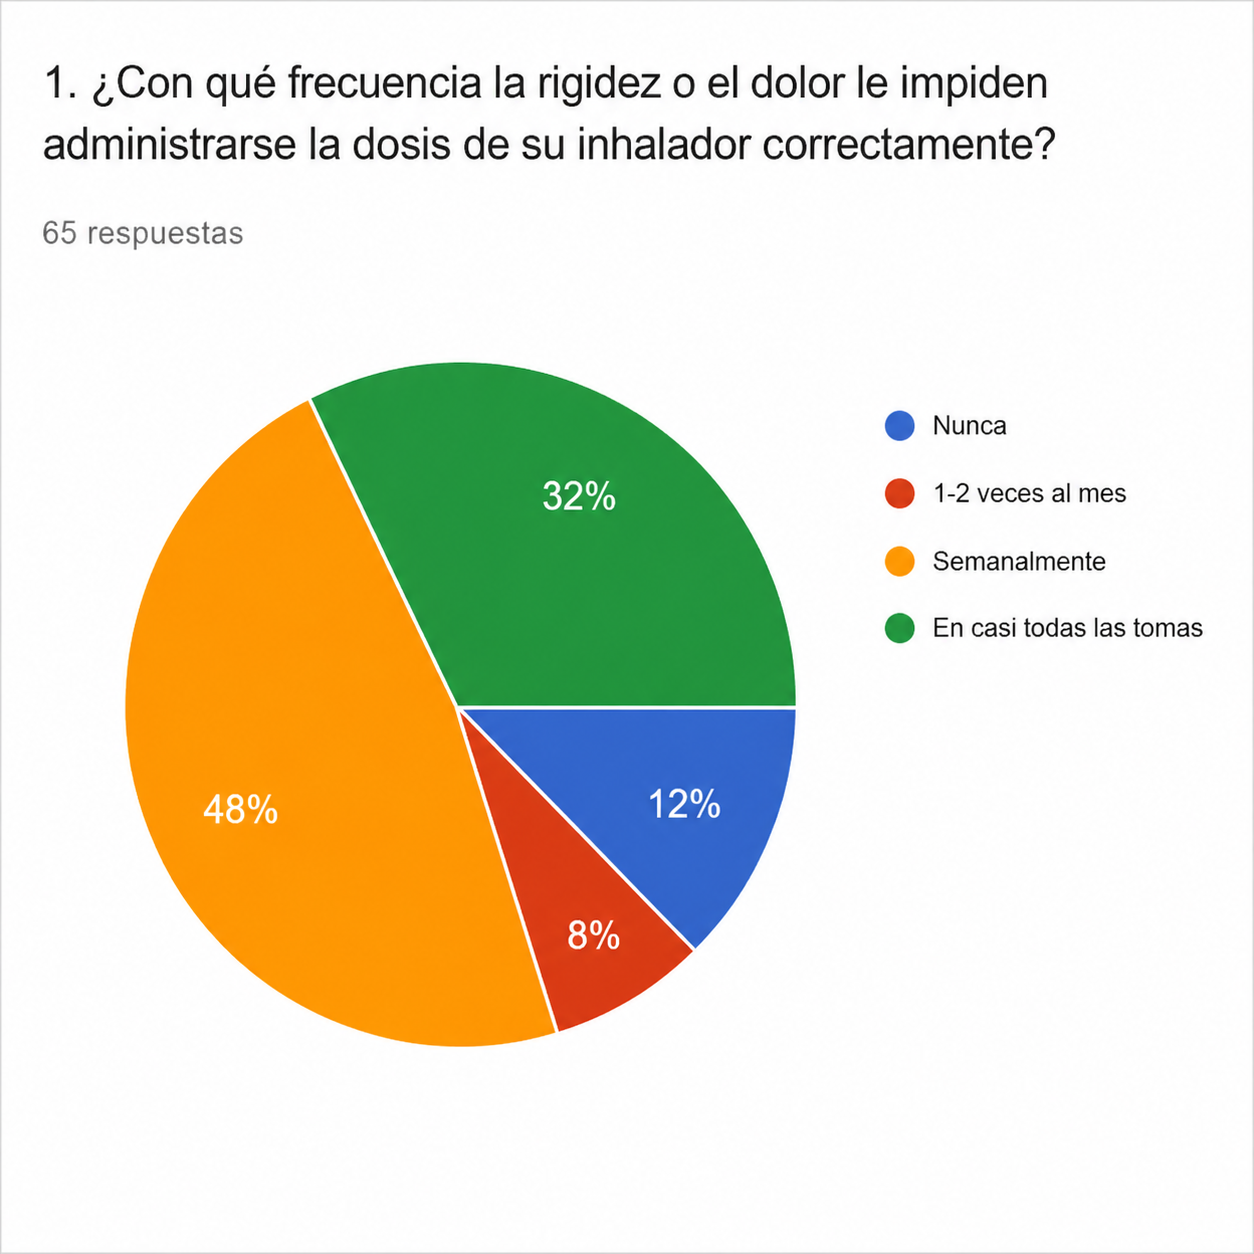
\includegraphics[width=6cm, trim=5bp 5bp 5bp 5bp, clip]{grafico1.png} \\ \hline
    \end{tabularx}
\end{table}

\vspace{0.4cm}

% --- RESULTADO 2 ---
\begin{table}[H]
    \centering
    \small
    \renewcommand{\tabularxcolumn}[1]{m{#1}}
    \begin{tabularx}{\linewidth}{|>{\raggedright\arraybackslash}X | >{\centering\arraybackslash}m{6.5cm}|}
        \hline
        \rowcolor{ArthroNavy}
        \multicolumn{2}{|l|}{\textcolor{white}{\textbf{2. Característica más importante en el accesorio ergonómico}}} \\ \hline
        \rowcolor{ArthroTeal!5}
        \vspace{0.2cm}
        \textbf{Distribución estadística:} \newline
        \textcolor{ArthroTeal}{\textbullet} \textbf{65\,\%:} Que reduzca el esfuerzo. \newline
        \textcolor{ArthroTeal}{\textbullet} \textbf{22\,\%:} Que sea fácil de colocar.\newline 
        \textcolor{ArthroTeal}{\textbullet} \textbf{8\,\%:} Que sea duradero. \newline\textcolor{ArthroTeal}{\textbullet} \textbf{5\,\%:} Que sea universal. 
        \vspace{0.4cm} \newline
        \textbf{Implicación técnica:} \newline
        El diseño debe centrarse en maximizar la ventaja mecánica por encima de cualquier otro factor estético o secundario.
        \vspace{0.2cm} & 
        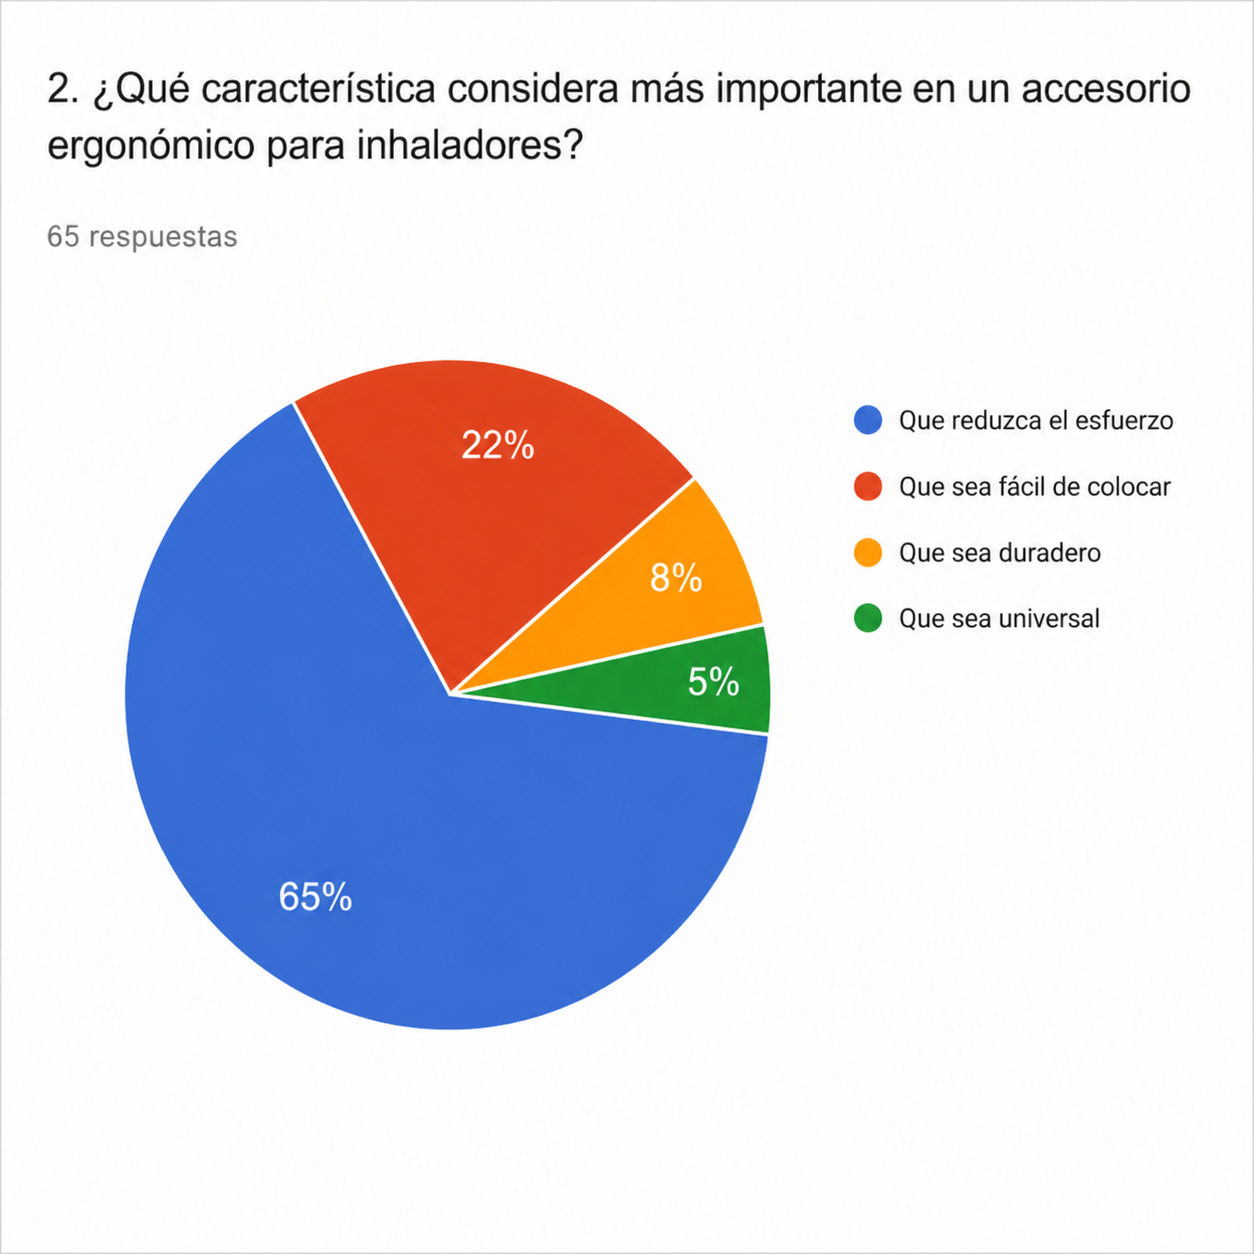
\includegraphics[width=6cm, trim=5bp 5bp 5bp 5bp, clip]{grafico2.png} \\ \hline
    \end{tabularx}
\end{table}

\vspace{0.4cm}

% --- RESULTADO 3 ---
\begin{table}[H]
    \centering
    \small
    \renewcommand{\tabularxcolumn}[1]{m{#1}}
    \begin{tabularx}{\linewidth}{|>{\raggedright\arraybackslash}X | >{\centering\arraybackslash}m{6.5cm}|}
        \hline
        \rowcolor{ArthroNavy}
        \multicolumn{2}{|l|}{\textcolor{white}{\textbf{3. Preferencia de superficie para la zona de agarre}}} \\ \hline
        \vspace{0.2cm}
        \textbf{Distribución estadística:} \newline
        \textcolor{ArthroTeal}{\textbullet} \textbf{58\,\%:} Rugosa/antideslizante. \newline
        \textcolor{ArthroTeal}{\textbullet} \textbf{30\,\%:} Blanda. \newline
        \textcolor{ArthroTeal}{\textbullet} \textbf{9\,\%:} Blanda. \newline
        \textcolor{ArthroTeal}{\textbullet} \textbf{3\,\%:} Sin preferencia.\vspace{0.4cm} \newline
         
        \textbf{Implicación técnica:} \newline
        Necesidad estricta de texturizar la zona de empuje palmar en los futuros moldes de inyección para asegurar la fricción.
        \vspace{0.2cm} & 
        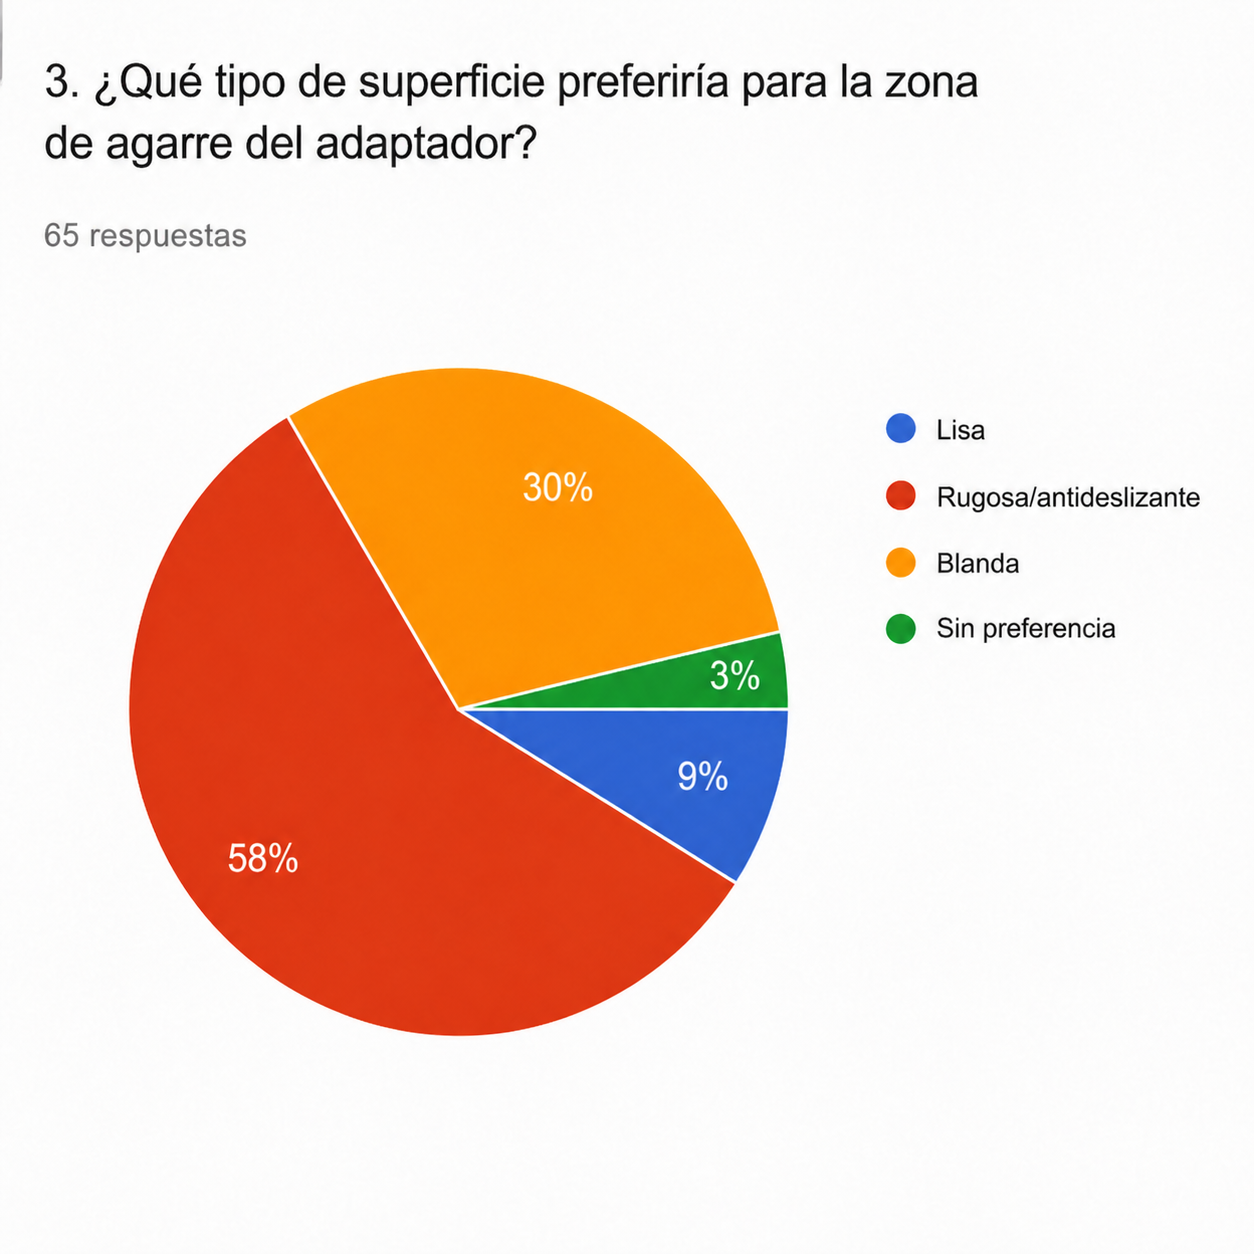
\includegraphics[width=6cm, trim=5bp 5bp 5bp 5bp, clip]{grafico3.png} \\ \hline
    \end{tabularx}
\end{table}

\vspace{0.4cm}

% --- RESULTADO 4 ---
\begin{table}[H]
    \centering
    \small
    \renewcommand{\tabularxcolumn}[1]{m{#1}}
    \begin{tabularx}{\linewidth}{|>{\raggedright\arraybackslash}X | >{\centering\arraybackslash}m{6.5cm}|}
        \hline
        \rowcolor{ArthroNavy}
        \multicolumn{2}{|l|}{\textcolor{white}{\textbf{4. Incremento de volumen aceptable para ganar comodidad}}} \\ \hline
        \rowcolor{ArthroTeal!5}
        \vspace{0.2cm}
        \textbf{Distribución estadística:} \newline
        \textcolor{ArthroTeal}{\textbullet} \textbf{62\,\%:} Aumento medio (bolso). \newline
        \textcolor{ArthroTeal}{\textbullet} \textbf{25\,\%:} Grande (uso doméstico).\newline
        \textcolor{ArthroTeal}{\textbullet} \textbf{13\,\%:} Muy compacto. \newline
        \vspace{0.4cm} \newline
        \textbf{Implicación técnica:} \newline
        La portabilidad de bolsillo estricta queda descartada, otorgando mayor libertad dimensional para diseñar el brazo de palanca.
        \vspace{0.2cm} & 
        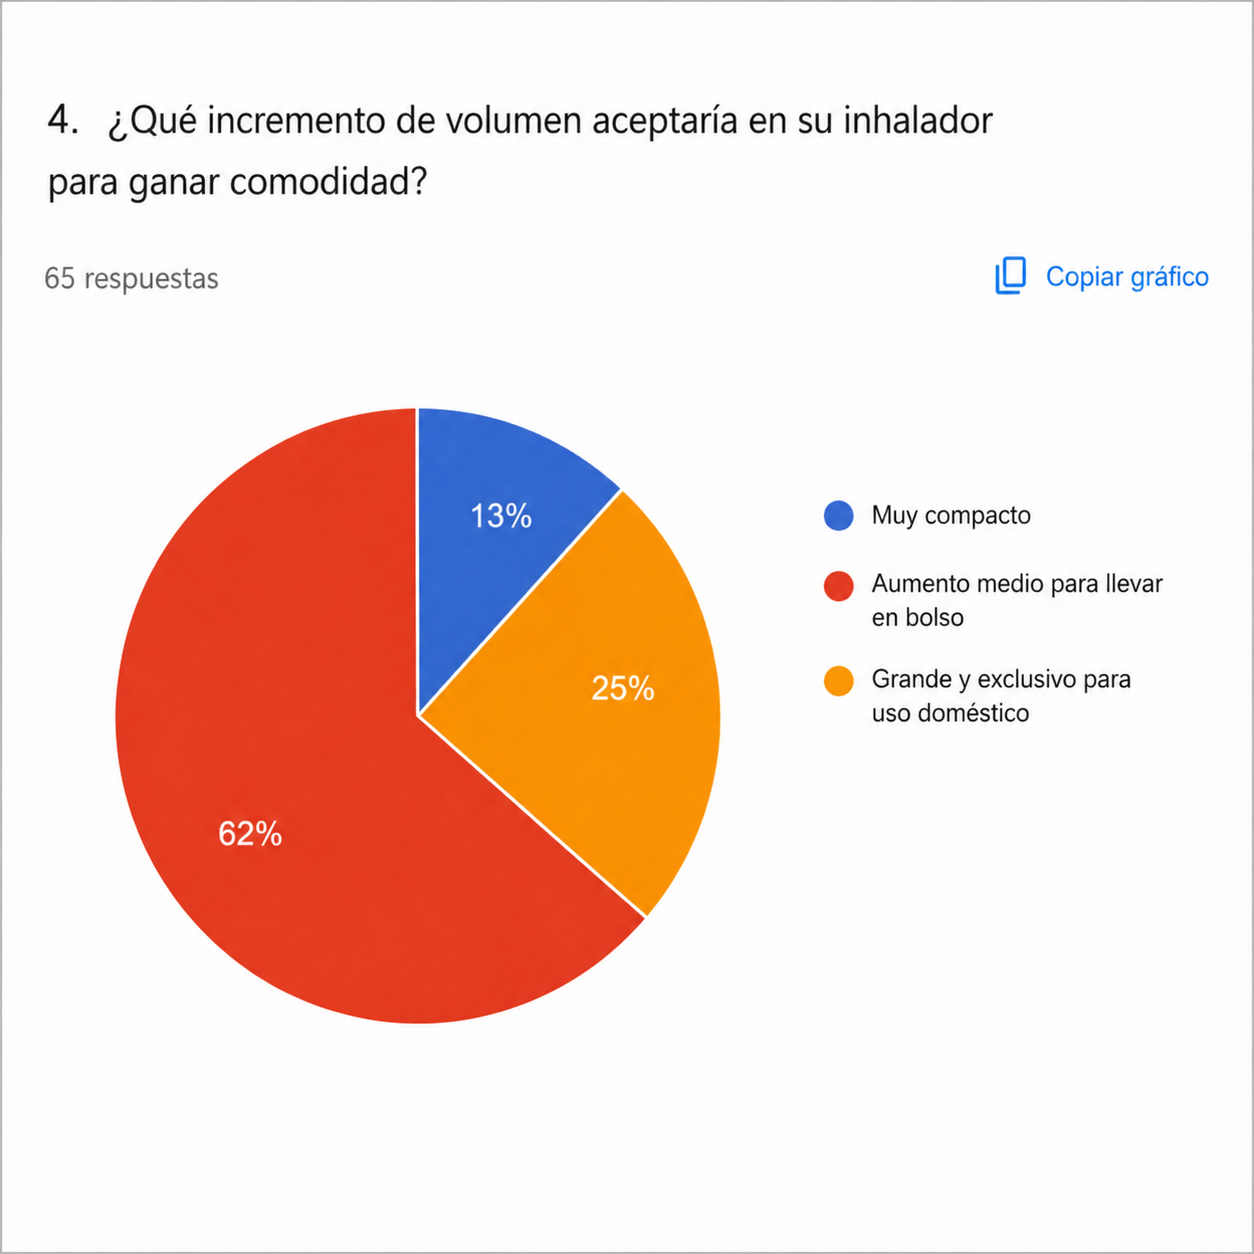
\includegraphics[width=6cm, trim=5bp 5bp 5bp 5bp, clip]{grafico4.png} \\ \hline
    \end{tabularx}
\end{table}

\vspace{0.4cm}

% --- RESULTADO 5 ---
\begin{table}[H]
    \centering
    \small
    \renewcommand{\tabularxcolumn}[1]{m{#1}}
    \begin{tabularx}{\linewidth}{|>{\raggedright\arraybackslash}X | >{\centering\arraybackslash}m{6.5cm}|}
        \hline
        \rowcolor{ArthroNavy}
        \multicolumn{2}{|l|}{\textcolor{white}{\textbf{5. Presupuesto máximo aceptable}}} \\ \hline
        \vspace{0.2cm}
        \textbf{Distribución estadística:} \newline
        \textcolor{ArthroTeal}{\textbullet} \textbf{54\,\%:} Entre 10€ y 20€. \newline
        \textcolor{ArthroTeal}{\textbullet} \textbf{30\,\%:} Menos de 10€. \newline
        \textcolor{ArthroTeal}{\textbullet} \textbf{12\,\%:} Entre 20€ y 35€.\newline
        \textcolor{ArthroTeal}{\textbullet} \textbf{4\,\%:} Más de 35€.
        \vspace{0.4cm} \newline
        \textbf{Implicación técnica:} \newline
        Este margen económico de venta obliga a optimizar la cantidad de piezas y simplificar el proceso de ensamblaje industrial.
        \vspace{0.2cm} & 
        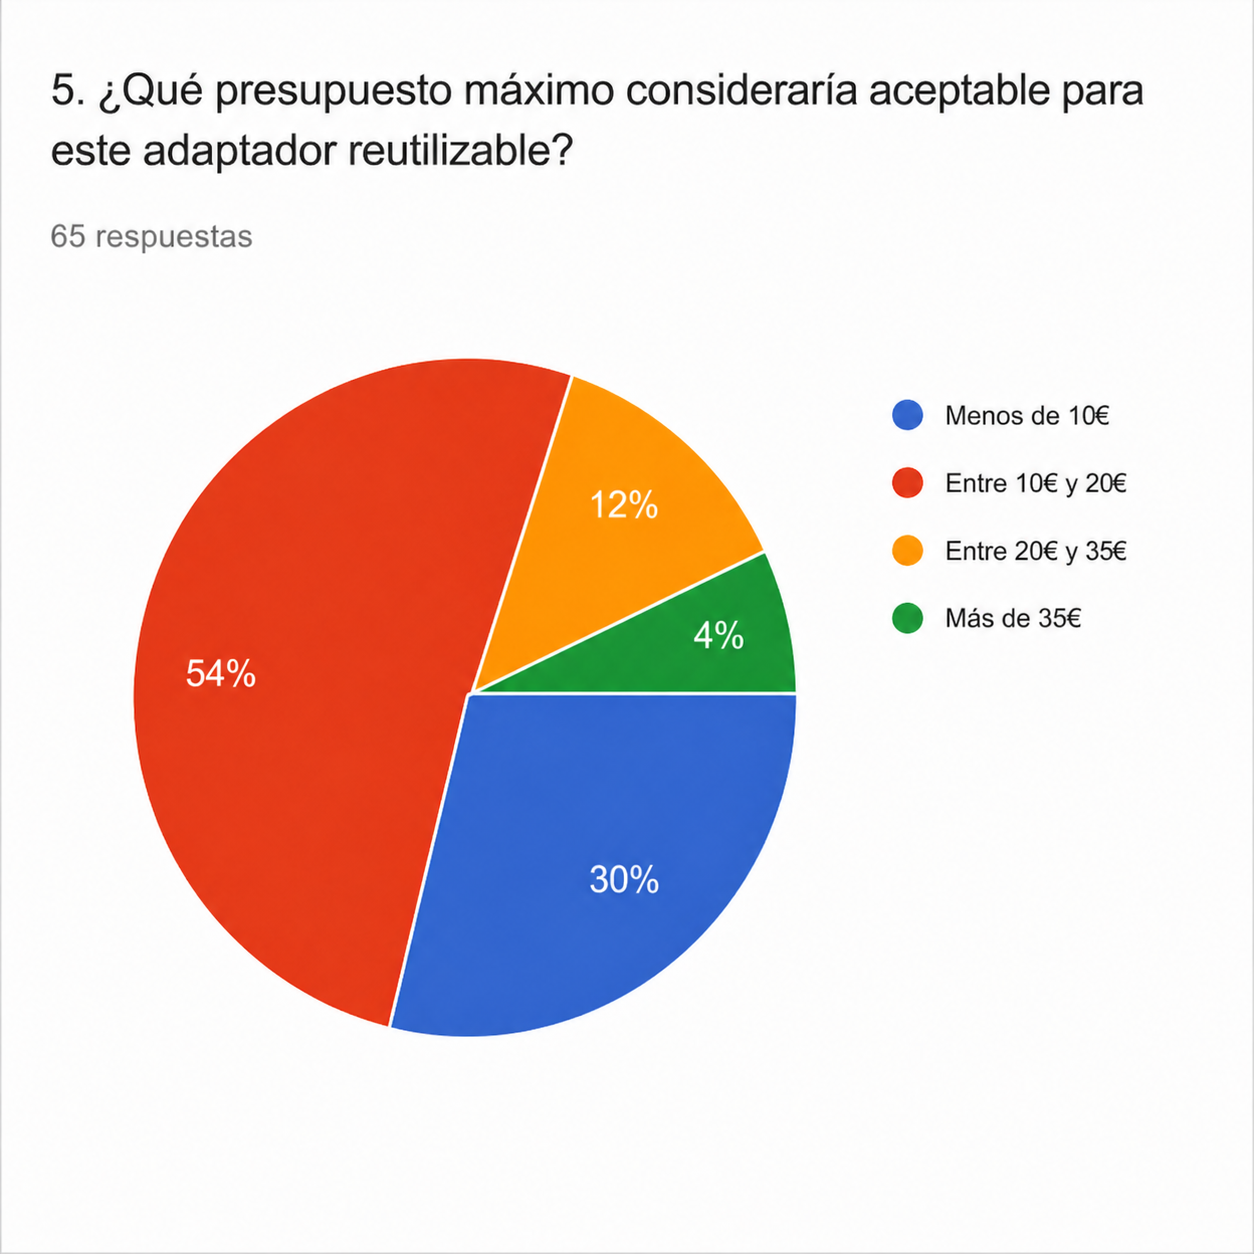
\includegraphics[width=6cm, trim=5bp 5bp 5bp 5bp, clip]{grafico5.png} \\ \hline
    \end{tabularx}
\end{table}
\newpage
\section{JUSTIFICACIÓN DE LAS DECISIONES}

\begin{table}[H]
    \centering
    \small
    \renewcommand{\arraystretch}{1.6}
    \renewcommand{\tabularxcolumn}[1]{m{#1}}
    \begin{tabularx}{\linewidth}{|>{\columncolor{ArthroNavy}\color{white}\bfseries\centering\arraybackslash}m{3.5cm} | X | X |}
        \hline
        \rowcolor{ArthroNavy}
        \multicolumn{1}{|c|}{\textcolor{white}{\textbf{Área de diseño}}} & 
        \multicolumn{1}{c|}{\textcolor{white}{\textbf{Origen y validación del dato}}} & 
        \multicolumn{1}{c|}{\textcolor{white}{\textbf{Decisión adoptada}}} \\ \hline
        
        Mecanismo y biomecánica & 
        \cellcolor{ArthroTeal!5}\textbf{Entrevista cualitativa:} \newline Declaraciones directas de la usuaria confirmando la incapacidad e intenso dolor al intentar flexionar los dedos. & 
        \cellcolor{ArthroTeal!5}Desarrollar una solución mecánica basada en el \textbf{principio de la palanca}, sustituyendo definitivamente el movimiento de pinza dactilar por un \textbf{empuje palmar} total. \\ \hline
        
        Dimensionamiento y estructura & 
        \textbf{Encuesta de mercado:} \newline Datos estadísticos que confirman una alta tolerancia al incremento del volumen del dispositivo si este mejora su uso. & 
        Descartar la miniaturización estricta. Se \textbf{prioriza la ergonomía estructural}, aprovechando el volumen extra aceptado para dimensionar un brazo de palanca eficiente. \\ \hline
        
        Viabilidad y mercado & 
        \cellcolor{ArthroTeal!5}\textbf{Estudio transversal:} \newline Evaluación conjunta del rango de presupuesto aceptable y las capacidades motoras de los pacientes. & 
        \cellcolor{ArthroTeal!5}Diseñar un adaptador que mantenga un bajo coste de fabricación industrial y un ensamblaje intuitivo sin necesidad de motricidad fina. \\ \hline
    \end{tabularx}
    \caption{Matriz de justificación técnica de las directrices de diseño extraídas del estudio de usuarios.}
    \label{tab:justificacion_decisiones}
\end{table}

\vspace{1.5cm}

 \vspace{0.5cm}
    \noindent\begin{minipage}{\textwidth}
    \begin{flushright}
        En Málaga, a \today
    \end{flushright}
    \vspace{2cm}

    \noindent
    \begin{minipage}[t]{0.45\textwidth}
        \centering
        \rule{6cm}{0.6pt} \\
        \textbf{Fdo. D. Sergio Carmona Muñoz} \\
        Colegiado Nº 06424 \\
        DNI: 26291930D
    \end{minipage}
    \hfill
    \begin{minipage}[t]{0.45\textwidth}
        \centering
        \rule{6cm}{0.6pt} \\
        \textbf{Fdo. D. Juan Gabriel Navarro Valdivielso} \\
        Colegiado Nº 06425 \\
        DNI: 77666662D
    \end{minipage}

    \vspace{2cm}

    \noindent
    \begin{minipage}[t]{0.45\textwidth}
        \centering
        \rule{6cm}{0.6pt} \\
        \textbf{Fdo. D. Antonio Sánchez Doña} \\
        Colegiado Nº 06423 \\
        DNI: 79380534J
    \end{minipage}
    \hfill
    \begin{minipage}[t]{0.45\textwidth}
        \centering
        \rule{6cm}{0.6pt} \\
        \textbf{Fdo. D. Iván de la Torre Segato} \\
        Colegiado Nº 06421 \\
        DNI: 79383630G
    \end{minipage}
\end{minipage}
    \vspace{1cm}

    % ======================================================
% HOJA EN BLANCO CON MARCA DE AGUA
% ======================================================
\newpage
\pagestyle{fancy}

\begin{tikzpicture}[remember picture, overlay]
    \node[opacity=0.1] at (current page.center) {
\includegraphics[width=12cm]{logo_definitivo.png}};
\end{tikzpicture}

% Empujamos el texto hacia la parte inferior del folio
\vspace*{8.5cm} 
\begin{center}
    \textit{Esta hoja ha sido dejada deliberadamente en blanco.}
\end{center}
\vfill


\end{document}

